\chapter{Аналитическая часть}

\section{Анализ предметной области}

\subsection{Социальный граф}

Строгое определение социального графа отсутствует, однако такие графы, как правило, обладают следующими свойствами:

\begin{enumerate}
	\item средняя длина пути между двумя произвольными вершинами невелика; типичным примером являются графы типа <<малого мира>>;
	\item для многих вершин выполняется следующее: если вершина A соединена с вершинами B и C, то с высокой вероятностью B и C также соединены между собой;
	\item граф содержит явно выраженные сообщества.
\end{enumerate}

\subsection{Сообщества}

Сообщество в социальном графе представляет собой подмножество вершин, между которыми плотность связей выше, чем с остальными вершинами графа. Примером такого сообщества может служить группа друзей в социальной сети.

\subsection{Модулярность}

Модулярность — это численная метрика, характеризующая качество разбиения графа на сообщества. Она определяется по формуле~(\ref{eq:modularity}):

\begin{equation}
	\label{eq:modularity}
	Q = \frac{1}{2m}\sum_{i,j}\left(A_{ij} - \frac{d_i d_j}{2m}\right)\delta(C_i, C_j),
\end{equation}

где $A_{ij}$ — элемент матрицы смежности, $d_i$ и $d_j$ — степени вершин $i$ и $j$, $m$ — общее количество рёбер в графе, $\delta(C_i, C_j)$ — индикаторная функция, равная единице, если вершины $i$ и $j$ принадлежат одному сообществу, и нулю в противном случае.

\section{Методы поиска сообществ на графах}

\subsection{Label Propagation}

Алгоритм Label Propagation основан на предположении, что вершина, большинство соседей которой принадлежат одному сообществу, с высокой вероятностью принадлежит этому же сообществу. В процессе работы каждая вершина присваивается тому сообществу, которому принадлежит наибольшее количество её соседей. В случае равного числа голосов выбор осуществляется случайным образом.

\subsection{Infomap}

Алгоритм Infomap~\cite{alg} базируется на концепции случайных блужданий по графу и кодировании траекторий с помощью кодов Хаффмана. Идея заключается в следующем: если использовать иерархическое кодирование, при котором сначала кодируется сообщество, а затем вершина внутри него, можно существенно сократить общую длину кода.

При входе в сообщество записывается его уникальный код, далее — код вершины. При перемещении внутри одного сообщества записываются только коды вершин. При выходе из сообщества фиксируется код выхода. Таким образом, алгоритм стремится минимизировать длину описания случайного блуждания.

\subsection{Edge Betweenness}

Edge Betweenness~\cite{alg} — это алгоритм, основанный на удалении рёбер с наибольшей центральностью. Для каждой пары вершин определяется множество кратчайших путей. Каждый такой путь делит единичный вес между всеми своими рёбрами. После обработки всех пар вершин каждому ребру сопоставляется значение, равное суммарному количеству проходящих через него кратчайших путей.

Затем из графа последовательно удаляются рёбра с наивысшими значениями edge betweenness. После удаления рёбер образуются компоненты связности, которые интерпретируются как сообщества. Итеративное применение процедуры позволяет построить иерархическую структуру разбиения графа.

\subsection{Louvain}

Алгоритм Louvain~\cite{louv} основан на жадной оптимизации модулярности~(\ref{eq:modularity}). На начальном этапе каждая вершина рассматривается как отдельное сообщество. Алгоритм включает два этапа:

\textbf{Первый этап:}
\begin{enumerate}
	\item для каждой вершины перебираются все соседние сообщества;
	\item вершина переносится в сообщество, при котором достигается максимальный прирост модулярности.
\end{enumerate}

\textbf{Второй этап:}
\begin{enumerate}
	\item строится мета-граф, в котором каждое сообщество представляется одной вершиной. Вес ребра между двумя такими вершинами равен суммарному весу рёбер между соответствующими сообществами. Рёбра внутри одного сообщества трансформируются в петлю;
	\item алгоритм повторяется с первого этапа.
\end{enumerate}

\subsection{Сравнение алгоритмов}

В таблице~\ref{tbl:srav_transposed} приведена сравнительная характеристика для алгоритмов поиска сообществ на графах.

\begin{table}[H]
	\begin{center}
		\begin{threeparttable}
			\caption{Сравнение алгоритмов обнаружения сообществ}
			\label{tbl:srav_transposed}
			\begin{tabularx}{\textwidth}{|X|X|X|X|p{2.7cm}|}
				\hline
				\textbf{Алгоритм} & \textbf{Работает с взвешенными графами} & \textbf{Работает с ориентированными графами} & \textbf{Не требует числа сообществ} & \textbf{Выявляет иерархические сообщества} \\
				\hline
				Label Propagation & + & - & + & - \\
				\hline
				Infomap           & + & + & + & + \\
				\hline
				Edge Betweenness  & + & - & - & -\\
				\hline
				Louvain           & + & - & + & + \\
				\hline
			\end{tabularx}
		\end{threeparttable}
	\end{center}
\end{table}

\subsection{Вывод}

Для описанной задачи в рамках курсовой был выбран алгоритм Louvain, так как он сочетает в себе высокую производительность, способность работать с взвешенными графами и автоматически выявляет иерархическую структуру сообществ. Алгоритм не требует предварительного указания количества кластеров и хорошо масштабируется на больших графах, что делает его подходящим для моделирования и анализа социальных сетей. Несмотря на то, что он не всегда гарантирует чёткие границы сообществ, его жадная оптимизация модулярности обеспечивает качественные результаты на практике.

\subsection{Формализация данных}

Для формального описания структуры используемых данных в рамках курсовой работы была выбрана графовая модель. В данной модели пользователи и сообщества представляются в виде вершин, а связи между ними — в виде рёбер.

Система формализуется как неориентированный взвешенный граф $G = (V, E)$, где:

\begin{itemize}
    \item $V$ — множество вершин. Вершины могут представлять как отдельных пользователей (\texttt{Person}), так и сообщества (\texttt{Community});
    \item $E$ — множество рёбер. Рёбра могут быть двух типов: связи между пользователями (\texttt{FRIENDS\_WITH}) и связи принадлежности пользователя к сообществу (\texttt{BELONGS\_TO});
    \item каждому ребру $e \in E$ может быть сопоставлен вес $w(e)$, отражающий силу связи. В текущей реализации вес по умолчанию равен 1.
\end{itemize}

Введены следующие сущности:

\begin{itemize}
    \item \textbf{Person (Человек)} — вершина, соответствующая пользователю социальной сети.
    \begin{itemize}
        \item \texttt{id}: уникальный идентификатор;
        \item \texttt{name}: имя пользователя;
        \item \texttt{level}: уровень иерархии (по умолчанию 0).
    \end{itemize}
    
    \item \textbf{Community (Сообщество)} — вершина, объединяющая пользователей на определённом уровне иерархии.
    \begin{itemize}
        \item \texttt{id}: уникальный идентификатор сообщества;
        \item \texttt{level}: уровень иерархии;
        \item \texttt{members}: список идентификаторов участников.
    \end{itemize}
    
    \item \textbf{FRIENDS\_WITH} — двунаправленная связь между двумя пользователями, отражающая их взаимодействие.
    \begin{itemize}
        \item \texttt{weight}: вес связи (по умолчанию 1).
    \end{itemize}
    
    \item \textbf{BELONGS\_TO} — направленная связь между пользователем и сообществом, указывающая на принадлежность.
\end{itemize}

На рисунке~\ref{fig:er} изображена диаграмма сущность -- связь.

\begin{figure}[H]
	\centering
	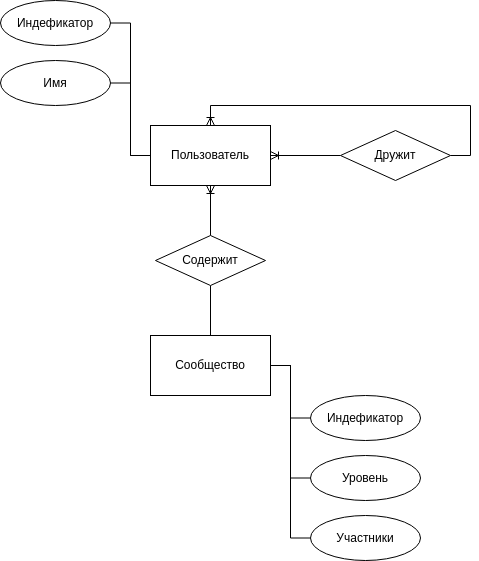
\includegraphics[height=0.4\textheight]{ER.png}
	\caption{Диаграмма сущность -- связь}
	\label{fig:er}
\end{figure}

\clearpage

На рисунке~\ref{fig:use-case} изображена диаграмма прецедентов.

\begin{figure}[H]
	\centering
	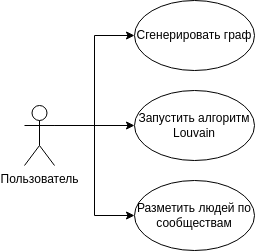
\includegraphics[height=0.3\textheight]{use-case.png}
	\caption{Диаграмма прецедентов}
	\label{fig:use-case}
\end{figure}

\section{Анализ типов баз данных}

\subsection{Дореляционные базы данных}

Дореляционные базы данных представляют собой системы управления, разработанные до появления реляционной модели. Наиболее распространённые типы:

\begin{itemize}
    \item \textbf{Иерархические СУБД} — организуют данные в древовидную структуру, где каждая запись имеет строго одного родителя (например, IBM IMS).
    \item \textbf{Сетевые СУБД} — обеспечивают более гибкие связи между записями в форме графа, что позволяет одной записи иметь несколько родителей.
\end{itemize}

Основные недостатки дореляционных моделей:
\begin{itemize}
    \item жёсткая и негибкая структура хранения данных;
    \item высокая степень связанности данных и прикладной логики;
    \item затруднённое масштабирование и модификация схем.
\end{itemize}

\subsection{Реляционные базы данных}

Реляционные СУБД основаны на модели, предложенной Э. Ф. Коддом в 1970 году. Данные представляются в виде таблиц (отношений), где строки соответствуют записям, а столбцы — атрибутам.

Преимущества реляционного подхода:
\begin{itemize}
    \item использование декларативного языка запросов SQL;
    \item логическая независимость данных от физической реализации;
    \item поддержка нормализации и формального анализа схем данных.
\end{itemize}

\subsection{Постреляционные базы данных}

Постреляционные базы данных развивают реляционную модель, объединяя её с объектно-ориентированными и семантическими концепциями. Такие СУБД сохраняют поддержку SQL, но дополнительно предоставляют:

\begin{itemize}
    \item хранение сложных структур данных (массивы, JSON, пользовательские типы);
    \item объектную иерархию и возможности интеграции с языками программирования;
    \item расширенные механизмы индексирования и обработки нетабличных данных.
\end{itemize}

\subsection{Графовые базы данных}

Графовые базы данных предназначены для хранения, обработки и анализа данных, представленных в виде графов. В отличие от реляционной модели, где основными единицами являются таблицы, в графовой модели основными сущностями выступают вершины (объекты) и рёбра (связи между объектами), при этом и те и другие могут содержать произвольные свойства (атрибуты).

Графовые СУБД особенно актуальны в задачах, где важна структура связей между сущностями, например:
\begin{itemize}
    \item социальные сети;
    \item рекомендательные системы;
    \item анализ связности и кластеризация;
    \item моделирование транспортных и телекоммуникационных сетей.
\end{itemize}

Преимущества графовых СУБД:
\begin{itemize}
    \item естественное представление сильно связанных данных;
    \item высокая производительность при выполнении многосвязных запросов (например, обходов в глубину или по шаблону);
\end{itemize}

\subsection{Сравнительная таблица}

В таблице~\ref{tbl:db_models} приведена сравнительная характеристика для видов баз данных.

\begin{table}[H]
	\begin{center}
		\begin{threeparttable}
			\caption{Сравнение моделей баз данных}
			\label{tbl:db_models}
			\begin{tabular}{|p{3cm}|p{3.5cm}|p{2.1cm}|p{2.9cm}|p{2.6cm}|}
				\hline
				Критерий & \makecell{Дореля-\\ционная} & \makecell{Реля-\\ционная} & \makecell{Постреля-\\ционная} & \makecell{Графовая} \\
				\hline
				Структура хранения & Иерархии или сети & Таблицы (отношения) & Таблицы + расширения & Граф (вершины и рёбра) \\
				\hline
				Тип связей & Жёстко заданные (один к одному/многим) & Через внешние ключи & Сложные структуры (JSON) & Явные рёбра между вершинами \\
				\hline
				Язык запросов & Собственные API & SQL & Расширенный SQL, объектные языки & Cypher, Gremlin и др. \\
				\hline
				Используется & Фиксированные структуры данных & Высокая согласованность данных & Разнородные данные & Сильно связные данные \\
				\hline
			\end{tabular}
		\end{threeparttable}
	\end{center}
\end{table}

\subsection{Вывод}

Для решения описанной ранее задачи подходит графовая СУБД. Так как социальная сеть является структурой с сильно связными данными. Так же графовая СУБД позволяет напрямую работать с графовой моделью данных, без создания отдельных таблиц. Язык запросов так же предназначен для работы с графовыми моделями данных, что является плюсом на фоне остальных СУБД.


\section*{Вывод}

В данном разделе была проанализирована предметная область, выбран алгоритм для поиска сообществ в графе и подходящий тип СУБД, для решения поставленной задачи.
